% The Krate Complete Guide
% Everything about Krate, in the simplest language that is still true.
% Written 2026-08-11. Every number in this document was measured or read
% out of the repository on that date. Nothing here is estimated.
\documentclass[11pt,a4paper]{report}

\usepackage[margin=2.4cm]{geometry}
\usepackage{fontspec}
\usepackage{titlesec}
\usepackage{xcolor}
\usepackage{booktabs}
\usepackage{longtable}
\usepackage{tabularx}
\usepackage{tikz}
\usepackage{hyperref}
\usepackage{fancyhdr}
\usepackage{enumitem}
\usepackage{tcolorbox}
\usetikzlibrary{shapes.geometric, arrows.meta, positioning, calc, fit, backgrounds}

\definecolor{krateblue}{HTML}{3B6BFF}
\definecolor{kratedark}{HTML}{0B1020}
\definecolor{krategrey}{HTML}{5A6472}
\definecolor{krategreen}{HTML}{1B8A5A}
\definecolor{kratered}{HTML}{C0392B}
\definecolor{kratebg}{HTML}{F4F6FA}

\hypersetup{colorlinks=true, linkcolor=krateblue, urlcolor=krateblue}

\titleformat{\chapter}[display]
  {\normalfont\huge\bfseries\color{krateblue}}
  {\chaptertitlename\ \thechapter}{12pt}{\Huge}
\titleformat{\section}
  {\normalfont\Large\bfseries\color{kratedark}}{\thesection}{1em}{}
\titleformat{\subsection}
  {\normalfont\large\bfseries\color{krategrey}}{\thesubsection}{1em}{}

\pagestyle{fancy}
\fancyhf{}
\fancyhead[L]{\small\color{krategrey}The Krate Complete Guide}
\fancyhead[R]{\small\color{krategrey}\thepage}
\renewcommand{\headrulewidth}{0.4pt}

\newtcolorbox{plainbox}[1]{colback=kratebg, colframe=krateblue,
  fonttitle=\bfseries, title={#1}, boxrule=0.6pt, arc=2pt}
\newtcolorbox{warnbox}[1]{colback=white, colframe=kratered,
  fonttitle=\bfseries, title={#1}, boxrule=0.6pt, arc=2pt}
\newtcolorbox{factbox}[1]{colback=white, colframe=krategreen,
  fonttitle=\bfseries, title={#1}, boxrule=0.6pt, arc=2pt}

\newcommand{\analogy}[1]{\begin{plainbox}{In everyday terms}#1\end{plainbox}}

\title{\vspace{-2cm}\Huge\textbf{Krate}\\[0.3cm]
  \Large The Complete Guide\\[0.6cm]
  \normalsize Everything about what it is, how it works, how it was built,\\
  and how to answer any question about it\\[1cm]}
\author{Krate Labs, Inc.}
\date{11 August 2026}

\begin{document}
\maketitle
\tableofcontents

% =====================================================================
\chapter{Read This First}

\section{What this document is}

This is one document that contains everything about Krate: what it is, why
it exists, how every piece works, how it was built, what went wrong along
the way, what the numbers actually are, and how to answer any question
anyone asks --- a curious friend, a developer, an investor, or a hostile
sceptic.

It assumes you know nothing. Not what WebAssembly is, not what Electron
is, not what a runtime is. Every technical idea is explained with an
example from ordinary life before any jargon appears.

\begin{factbox}{The rule this document follows}
Every number here was measured on 11 August 2026, or read directly out of
the repository on that date. Where something is unknown, this document
says it is unknown. Where a number depends on conditions, the conditions
are stated. Nothing is estimated, rounded up, or assumed.
\end{factbox}

\section{Krate in five sentences}

\begin{enumerate}[leftmargin=*]
  \item An AI can now write you a working desktop app in a few minutes.
  \item But you cannot easily \emph{give} that app to anyone --- they would
    need the right programming languages installed, or a 200-megabyte
    bundle, or they will see a scary security warning.
  \item Krate turns that app into \textbf{one small file}, typically 15 to
    30 kilobytes, that opens by double-click on macOS, Windows and Linux.
  \item Before the app runs, it says in plain words what it wants to touch
    (``save files in its own private folder --- never your files''), and
    the runtime \emph{enforces} that, so an app cannot exceed what you
    allowed.
  \item You send it like you would send a photo, or publish it and send a
    link.
\end{enumerate}

\analogy{Think of a PDF. Before PDFs, sending someone a document meant
hoping they had the same word processor, the same version, and the same
fonts. The PDF made a document \emph{one file that just opens}. Krate is
trying to be the PDF of small applications.}

% =====================================================================
\chapter{The Basics, Explained From Zero}

This chapter assumes no technical knowledge at all. If you already know
what WebAssembly and sandboxing are, you can skip to Chapter 3 --- but
this chapter is also the source of the analogies you should use when
explaining Krate to other people.

\section{What is a program, really?}

A program is a list of instructions for a machine. But a computer's
processor does not understand English, or Python, or any language a person
writes in. It understands only \textbf{machine code} --- numbers that mean
``add these'', ``store this here'', ``jump there''.

So there is always a translation step:

\begin{center}
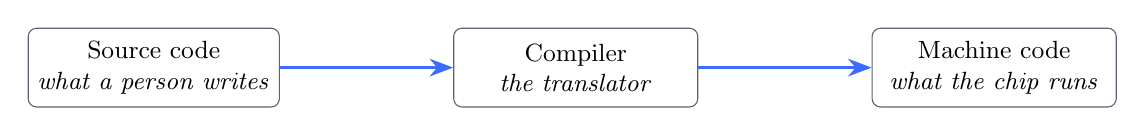
\begin{tikzpicture}[node distance=1.6cm and 2.2cm,
  box/.style={draw=krategrey, rounded corners=3pt, fill=white,
    minimum width=3.1cm, minimum height=1cm, align=center, font=\small},
  arrow/.style={-{Stealth[length=3mm]}, thick, draw=krateblue}]
  \node[box] (src) {Source code\\\textit{what a person writes}};
  \node[box, right=of src] (comp) {Compiler\\\textit{the translator}};
  \node[box, right=of comp] (mach) {Machine code\\\textit{what the chip runs}};
  \draw[arrow] (src) -- (comp);
  \draw[arrow] (comp) -- (mach);
\end{tikzpicture}
\end{center}

\subsection{Why the same app does not run everywhere}

Here is the problem that has existed since computers began: \textbf{machine
code is different on every kind of computer.}

A Mac with an Apple chip speaks one dialect (called \texttt{arm64}). An
older Mac or most Windows PCs speak another (\texttt{x86\_64}). And even
on the same chip, macOS, Windows and Linux each expect programs to be
packaged differently and to ask for files and windows in different ways.

\analogy{It is like electrical plugs. The electricity is the same idea
everywhere, but the plug shape is different in the UK, the US and India.
A device built for one socket physically cannot go into another.}

So historically, if you wrote an app and wanted everyone to run it, you had
to build it three times, test it three times, and ship three different
files. That is expensive, and it is why most small useful programs never
get shared at all.

\section{The four ways people have solved this, and what each costs}

\subsection{Way 1: Build it separately for each system (``native'')}

Write the app, then compile it once for Mac, once for Windows, once for
Linux. Three builds, three files, three sets of bugs.

\begin{itemize}[leftmargin=*]
  \item \textbf{Good:} fastest possible, feels exactly like the system it
    runs on.
  \item \textbf{Bad:} three times the work, forever. And the person
    receiving it still gets security warnings, because the operating
    system does not know who you are.
\end{itemize}

\subsection{Way 2: Ship a whole web browser with your app (``Electron'')}

This is what Slack, Discord, VS Code and Notion do. The app is really a
web page, and the ``app'' you download contains an entire copy of the
Chrome browser to display that web page.

\begin{itemize}[leftmargin=*]
  \item \textbf{Good:} write once, runs everywhere, and web developers can
    build it.
  \item \textbf{Bad:} enormous. A tool that does something simple arrives
    as 80 to 200 megabytes, uses a lot of memory, and starts slowly.
\end{itemize}

\analogy{It is like mailing someone a letter, but because you are not sure
they own reading glasses, you post them a pair of glasses with every
letter. It works, but the envelope is now enormous, and they now have
forty pairs of glasses.}

\subsection{Way 3: Make it a website instead}

Do not ship anything; put it on the internet and send a link.

\begin{itemize}[leftmargin=*]
  \item \textbf{Good:} nothing to install, works on everything.
  \item \textbf{Bad:} you do not own it, it needs internet, it cannot
    easily touch your own files, and it disappears the day someone stops
    paying the hosting bill.
\end{itemize}

\subsection{Way 4: A shared runtime (this is where Krate lives)}

Ship the app in \emph{one} portable format, and put a small program on
each computer that knows how to run that format.

This idea is old and proven: it is how Java worked, and how a PDF reader
works. The app file is the same everywhere; the thing that reads it is
built for each system.

\begin{center}
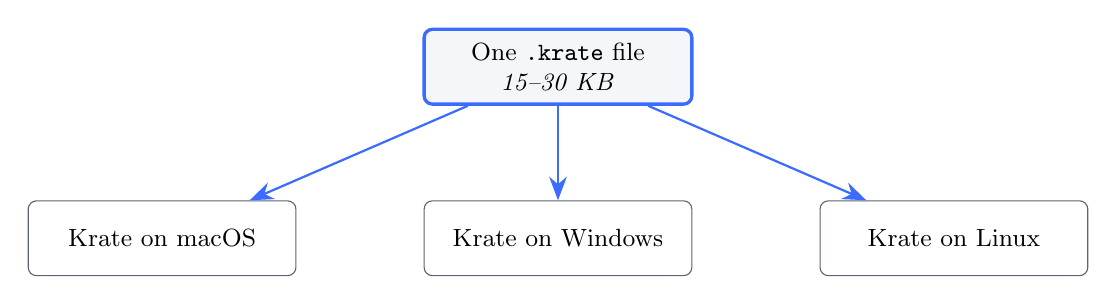
\begin{tikzpicture}[node distance=1.2cm and 1.6cm,
  box/.style={draw=krategrey, rounded corners=3pt, fill=white,
    minimum width=3.4cm, minimum height=0.95cm, align=center, font=\small},
  kbox/.style={draw=krateblue, very thick, rounded corners=3pt, fill=kratebg,
    minimum width=3.4cm, minimum height=0.95cm, align=center, font=\small},
  arrow/.style={-{Stealth[length=3mm]}, thick, draw=krateblue}]
  \node[kbox] (file) {One \texttt{.krate} file\\\textit{15--30 KB}};
  \node[box, below left=of file] (mac) {Krate on macOS};
  \node[box, below=of file] (win) {Krate on Windows};
  \node[box, below right=of file] (lin) {Krate on Linux};
  \draw[arrow] (file) -- (mac);
  \draw[arrow] (file) -- (win);
  \draw[arrow] (file) -- (lin);
\end{tikzpicture}
\end{center}

\section{What is WebAssembly?}

WebAssembly (usually written \textbf{Wasm}) is a portable form of machine
code. It was invented so that web browsers could run fast programs written
in languages other than JavaScript, but it turned out to be useful far
beyond browsers.

Three properties matter for Krate:

\begin{enumerate}[leftmargin=*]
  \item \textbf{It is portable.} One Wasm file runs on any chip and any
    operating system that has a Wasm runtime.
  \item \textbf{It is fast.} It is real compiled code, not an interpreted
    script. It runs at close to native speed.
  \item \textbf{It is sandboxed by design.} This is the crucial one. A Wasm
    program \emph{cannot do anything at all} on its own --- it cannot open
    a file, reach the network, or draw on the screen. It can only do what
    the runtime around it explicitly hands over.
\end{enumerate}

\analogy{A normal program is a guest with the run of your house. A Wasm
program is a guest in a room with no doors --- the only things it can
reach are what you deliberately pass through a hatch. That is not a
restriction someone added afterwards; it is how the room is built.}

That third property is why Krate can make a promise no ordinary app can
make. The permission wall is not politeness. The app genuinely has no way
to reach anything you did not grant.

\section{What is a ``runtime''?}

A runtime is the program that runs other programs.

When you double-click a \texttt{.krate} file, you are not running the app
directly --- your operating system runs \textbf{Krate}, and Krate reads the
app and runs it inside itself, deciding what the app is allowed to do.

\analogy{A runtime is a games console. The disc holds the game, but the
disc cannot do anything by itself. The console reads it, runs it, and
controls what the game can reach --- the screen, the controller, the memory
card. The same disc works in any console of that type, anywhere in the
world.}

\begin{plainbox}{So what is ``the Krate runtime''?}
It is a single program, about 21 megabytes, that you install once. It
contains: a WebAssembly engine (\texttt{wasmtime}), a permission checker,
a drawing system that can paint windows on three operating systems, and
everything else an app might legitimately need --- a clock, a filesystem
gate, a network gate, a key-value store, a database, sound, and text
rendering.
\end{plainbox}

% =====================================================================
\chapter{What Krate Actually Is}

\section{The one-sentence version}

\begin{plainbox}{Krate}
Krate makes an AI-written app into one small file that runs on any
computer, tells you what it wants before it runs, and cannot do anything
you did not allow.
\end{plainbox}

\section{The problem, stated precisely}

The making of software just got solved. Anyone can now ask an AI for a
tool and get working code in minutes. But the \emph{delivering} of software
did not change at all:

\begin{itemize}[leftmargin=*]
  \item If your AI writes Python, the person you send it to needs Python
    installed, and the right version, and the libraries.
  \item If it writes a web app, someone must host it, forever.
  \item If it writes a native app, it must be built three times, and it
    will still trigger security warnings on arrival.
  \item If it wraps a browser (Electron), a two-hundred-line tool becomes a
    two-hundred-megabyte download.
\end{itemize}

And beneath all of that is a trust problem: \textbf{why would you run a
program a stranger's AI wrote?} You cannot read the code. You have no idea
what it touches.

\section{The three things Krate does about it}

\subsection{One file that runs anywhere}

A Krate app is one \texttt{.krate} file. Measured examples from the live
gallery on 11 August 2026:

\begin{center}
\begin{tabular}{lr}
\toprule
\textbf{App} & \textbf{Size} \\
\midrule
``Sadas'' (published by a user) & 14{,}974 bytes \\
``Add dvd screensaver'' & 15{,}135 bytes \\
``World Clock'' & 24{,}261 bytes \\
``Journal'' & 29{,}878 bytes \\
Breakout game (playable, in-repo) & 31{,}455 bytes \\
\bottomrule
\end{tabular}
\end{center}

For comparison, the same kind of tool built with Electron is typically
80--200 megabytes. A 30-kilobyte game is roughly \textbf{five thousand
times smaller} than a 150-megabyte Electron app.

\subsection{A permission wall that is real}

Before an app runs, the person sees what it wants, in the app's own words:

\begin{verbatim}
    Krategram wants to:

      Open the feed window                    [on]
        ui.window:create

      Print progress markers                  [on]
        io.stdout

              [ Open ]        Cancel
\end{verbatim}

Two things make this different from the permission prompts you are used
to:

\begin{enumerate}[leftmargin=*]
  \item \textbf{Denying still opens the app.} Turn something off and the
    app runs without that power, rather than refusing to start.
  \item \textbf{It is enforced by the machine, not by policy.} The app
    physically cannot call what it was not granted --- the check happens at
    the boundary between the app and the runtime, on every single call.
\end{enumerate}

\subsection{The AI writes it, and a machine checks the AI's work}

You type what you want in plain words. Whichever AI you already pay for
(Claude, Codex, Gemini, Copilot, Grok) writes real compiled code. Then
Krate's own checker --- \texttt{check-app} --- builds it, verifies it only
uses Krate's APIs, runs it, resizes its window, clicks it, and watches
whether it closes itself. Only then do you get a file.

\section{The idea that impresses engineers most: ``the pick is the grant''}

Consider an app that tidies your Downloads folder. Every other system
solves this by asking for broad filesystem access --- and then you are
trusting it.

In Krate, such an app \textbf{cannot name a folder at all}. There is no
capability it can declare that would let it. Instead it asks you to pick
one. Your pick becomes the permission: scoped to that folder, for that run
only, and gone when the app closes.

\begin{center}
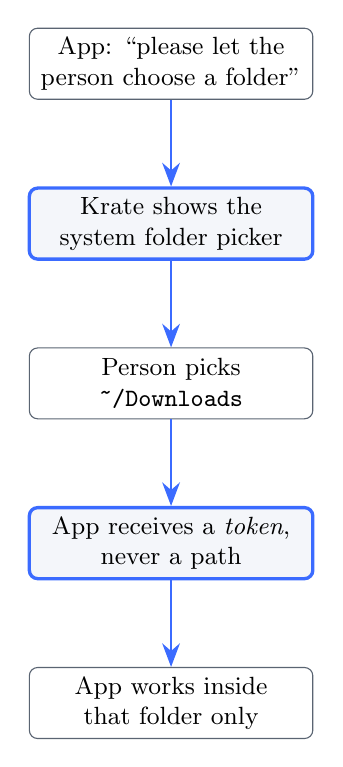
\begin{tikzpicture}[node distance=1.1cm and 1.5cm,
  box/.style={draw=krategrey, rounded corners=3pt, fill=white,
    minimum width=3.6cm, minimum height=0.9cm, align=center, font=\small},
  kbox/.style={draw=krateblue, very thick, rounded corners=3pt, fill=kratebg,
    minimum width=3.6cm, minimum height=0.9cm, align=center, font=\small},
  arrow/.style={-{Stealth[length=3mm]}, thick, draw=krateblue}]
  \node[box] (a) {App: ``please let the\\person choose a folder''};
  \node[kbox, below=of a] (b) {Krate shows the\\system folder picker};
  \node[box, below=of b] (c) {Person picks\\\texttt{\textasciitilde/Downloads}};
  \node[kbox, below=of c] (d) {App receives a \emph{token},\\never a path};
  \node[box, below=of d] (e) {App works inside\\that folder only};
  \draw[arrow] (a) -- (b);
  \draw[arrow] (b) -- (c);
  \draw[arrow] (c) -- (d);
  \draw[arrow] (d) -- (e);
\end{tikzpicture}
\end{center}

The working example ships in the repository as \texttt{apps/krate-tidy}.
Its manifest declares \textbf{zero} filesystem capabilities.

\analogy{It is the difference between giving a builder the keys to your
house, and walking them to one room and standing there while they work.}

% =====================================================================
\chapter{How Krate Works Inside}

\section{The whole system on one page}

\begin{center}
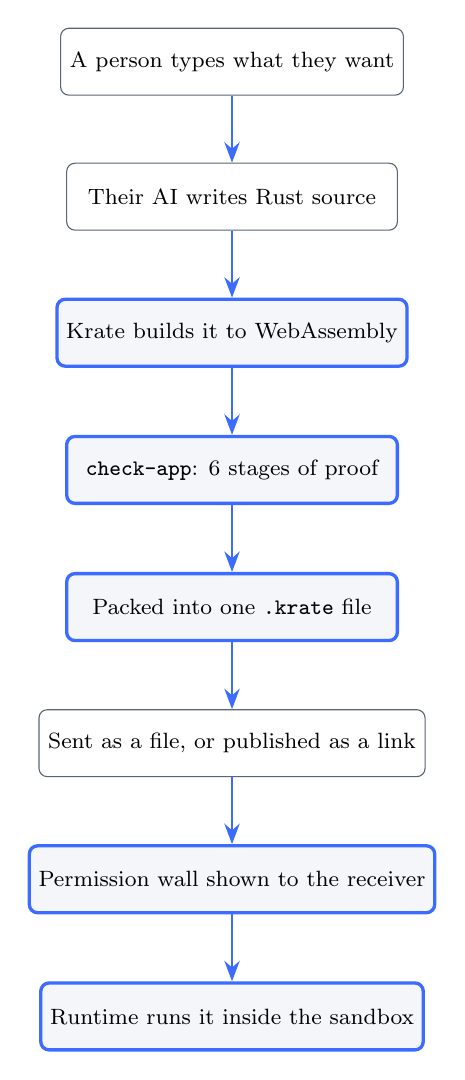
\begin{tikzpicture}[node distance=0.85cm and 1.3cm,
  box/.style={draw=krategrey, rounded corners=3pt, fill=white,
    minimum width=4.2cm, minimum height=0.85cm, align=center, font=\footnotesize},
  kbox/.style={draw=krateblue, very thick, rounded corners=3pt, fill=kratebg,
    minimum width=4.2cm, minimum height=0.85cm, align=center, font=\footnotesize},
  arrow/.style={-{Stealth[length=2.6mm]}, thick, draw=krateblue}]

  \node[box] (person) {A person types what they want};
  \node[box, below=of person] (ai) {Their AI writes Rust source};
  \node[kbox, below=of ai] (build) {Krate builds it to WebAssembly};
  \node[kbox, below=of build] (check) {\texttt{check-app}: 6 stages of proof};
  \node[kbox, below=of check] (pack) {Packed into one \texttt{.krate} file};
  \node[box, below=of pack] (share) {Sent as a file, or published as a link};
  \node[kbox, below=of share] (wall) {Permission wall shown to the receiver};
  \node[kbox, below=of wall] (run) {Runtime runs it inside the sandbox};

  \draw[arrow] (person) -- (ai);
  \draw[arrow] (ai) -- (build);
  \draw[arrow] (build) -- (check);
  \draw[arrow] (check) -- (pack);
  \draw[arrow] (pack) -- (share);
  \draw[arrow] (share) -- (wall);
  \draw[arrow] (wall) -- (run);
\end{tikzpicture}
\end{center}

\section{What is inside the runtime}

Krate is 112{,}860 lines of Rust across 20 components. The largest pieces,
measured on 11 August 2026:

\begin{center}
\begin{longtable}{lrp{7.4cm}}
\toprule
\textbf{Component} & \textbf{Lines} & \textbf{What it does} \\
\midrule
\endhead
\texttt{cli} & 23{,}764 & The \texttt{krate} command: run, create, check, pack, publish, doctor \\
\texttt{runtime} & 22{,}483 & Runs apps, enforces permissions, draws canvases \\
\texttt{tools} & 8{,}077 & Internal development and verification tooling \\
\texttt{adapter-common} & 8{,}032 & Shared drawing and text rendering \\
\texttt{bindings-rust} & 6{,}534 & The SDK an app is written against \\
\texttt{adapter-macos} & 5{,}598 & Native windows on macOS \\
\texttt{adapter-ios} & 3{,}109 & iPhone windows and GPU rendering \\
\texttt{author} & 2{,}723 & Drives the AI that writes apps \\
\texttt{port} & 2{,}644 & Analyses existing projects for portability \\
\texttt{mcp} & 2{,}633 & Lets a chat model build apps by talking \\
\texttt{adapter-android} & 2{,}258 & Android windows and touch \\
\texttt{adapter-windows} & 2{,}008 & Native windows on Windows \\
\texttt{adapter-linux} & 1{,}987 & Native windows on Linux \\
\texttt{layout} & 1{,}393 & Arranges things on screen \\
\texttt{bundle} & 1{,}385 & Reads and writes the \texttt{.krate} file format \\
\texttt{manifest} & 1{,}212 & Parses and validates what an app asks for \\
\texttt{krate-hub} & 513 & The cloud service \\
\texttt{policy} & 494 & Decides what is granted \\
\texttt{player-android} & 420 & The Android app that opens \texttt{.krate} files \\
\texttt{player-ios} & 240 & The iPhone app that opens \texttt{.krate} files \\
\bottomrule
\end{longtable}
\end{center}

\section{How the permission wall actually works}

There are three layers, and all three must agree. This matters, because we
learned the hard way that two out of three is the same as zero.

\begin{center}
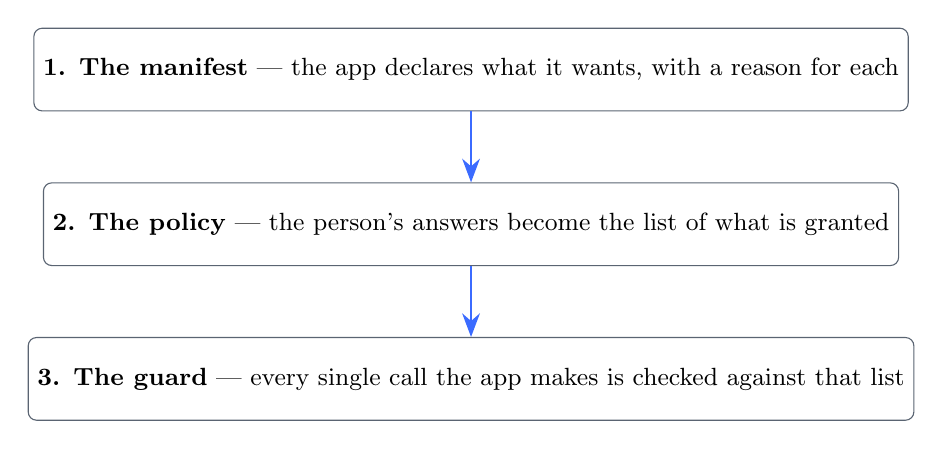
\begin{tikzpicture}[node distance=0.9cm,
  box/.style={draw=krategrey, rounded corners=3pt, fill=white,
    minimum width=10cm, minimum height=1.05cm, align=left, font=\small},
  arrow/.style={-{Stealth[length=3mm]}, thick, draw=krateblue}]
  \node[box] (m) {\textbf{1. The manifest} --- the app declares what it wants,
    with a reason for each};
  \node[box, below=of m] (p) {\textbf{2. The policy} --- the person's answers
    become the list of what is granted};
  \node[box, below=of p] (g) {\textbf{3. The guard} --- every single call the app
    makes is checked against that list};
  \draw[arrow] (m) -- (p);
  \draw[arrow] (p) -- (g);
\end{tikzpicture}
\end{center}

In August 2026 we found (bug K-086) that the third layer was missing for
dialog boxes: the wall showed the words, the policy recorded the answer,
and nothing checked it. Any app could open file pickers it had never asked
for. All three layers now carry their own test.

\section{The six checks every app must pass}

\texttt{check-app} is the machine that decides whether an app is real. An
AI writes code, this decides whether the code is acceptable, and the AI
tries again until it passes.

\begin{center}
\begin{tabular}{clp{8.6cm}}
\toprule
& \textbf{Stage} & \textbf{What it proves} \\
\midrule
1 & layout & The three required files exist and the code is not obviously wrong \\
2 & manifest & Everything it asks for is real, scoped, and actually used by the code \\
3 & build & It compiles to WebAssembly \\
4 & imports & It uses \emph{only} Krate APIs --- no smuggled operating-system access \\
5 & run & It actually runs, headless, without crashing \\
6 & usability & Its window opens, survives a resize, responds to a click, and does not close itself \\
\bottomrule
\end{tabular}
\end{center}

Stage 6 is unusual and it is the one that catches what people actually
complain about. On 11 August 2026 it caught 21 of our own 32 example apps
drawing at a fixed size and ignoring the window --- the exact bug a
first-time user reported from Windows.

% =====================================================================
\chapter{The Complete Technical Reference}

This chapter is the deep detail: the exact capability list, the exact file
format, the exact commands, and the exact release pipeline. You do not need
to memorise it. You need to know it exists so that when somebody asks a
specific question, the answer is here.

\section{The capability list, complete}

There are exactly \textbf{37} capabilities. \textbf{14} are granted to every
app automatically; \textbf{23} must be explicitly asked for, appear on the
permission wall, and can be refused.

The dividing principle is simple and worth being able to state: \emph{a
capability is granted by default only if using it moves no data and takes
no outward action.} Reading the clock moves no data. Reading your clipboard
does. Showing a message box takes no outward action. Sending a desktop
notification does.

\subsection{Granted to every app (14)}

\begin{center}
\begin{tabular}{llp{6.6cm}}
\toprule
\textbf{Capability} & \textbf{Phase} & \textbf{Why it needs no permission} \\
\midrule
\texttt{io.stdin} & 2 & Text in and out of the app's own terminal \\
\texttt{io.stdout} & 2 & \\
\texttt{io.stderr} & 2 & \\
\texttt{io.args} & 2 & The arguments it was started with \\
\texttt{io.log} & 2 & Its own diagnostic output \\
\texttt{time.clock} & 2 & What time it is reveals nothing \\
\texttt{time.monotonic} & 2 & How long something took \\
\texttt{time.sleep} & 2 & Waiting \\
\texttt{locale.info} & 2 & Your language and region \\
\texttt{locale.format} & 2 & Formatting a date the local way \\
\texttt{ui.window:create} & 3 & An app with a window is the normal case \\
\texttt{ui.dialog:message} & 3 & Shows text; no data moves \\
\texttt{ui.dialog:confirm} & 3 & Takes a click; no data moves \\
\texttt{gfx.gpu:basic} & 3 & Drawing inside its own window \\
\bottomrule
\end{tabular}
\end{center}

\subsection{Must be asked for (23)}

\begin{center}
\begin{longtable}{llp{6.4cm}}
\toprule
\textbf{Capability} & \textbf{Phase} & \textbf{What it lets the app do} \\
\midrule
\endhead
\texttt{fs.read:<glob>} & 2 & Read files matching a pattern \\
\texttt{fs.write:<glob>} & 2 & Write files matching a pattern \\
\texttt{fs.list:<glob>} & 2 & See what files exist \\
\texttt{fs.remove:<glob>} & 2 & Delete files \\
\texttt{fs.mkdir:<glob>} & 2 & Create folders \\
\texttt{net.connect:<host>:<port>} & 2 & Reach one named host and port --- not ``the internet'' \\
\texttt{store.kv} & 2 & Remember things between runs \\
\texttt{store.sql} & 2 & Keep its own database \\
\texttt{store.secret} & 2 & Keep tokens and keys, encrypted at rest \\
\texttt{random.bytes} & 2 & Draw random numbers \\
\texttt{ui.clipboard:read} & 3 & Read what you copied \\
\texttt{ui.clipboard:write} & 3 & Put something on your clipboard \\
\texttt{ui.menu:system} & 3 & Add to the system menu bar \\
\texttt{ui.open-url} & 3 & Hand a link to your browser \\
\texttt{ui.notify} & 3 & Send a desktop notification \\
\texttt{ui.dropzone:<mime>} & 3 & Accept files dragged onto it \\
\texttt{ui.dialog:file-open} & 3 & Ask you to pick a file to open \\
\texttt{ui.dialog:file-save} & 3 & Ask you where to save \\
\texttt{ui.dialog:open-folder} & 3 & Ask you to pick a folder --- the biggest dialog grant \\
\texttt{ui.dialog:*} & 3 & All dialogs at once \\
\texttt{gfx.gpu:compute} & 3 & General-purpose GPU work (not implemented yet) \\
\texttt{audio.playback} & 3 & Make sound \\
\texttt{audio.capture} & 3 & Use your microphone \\
\bottomrule
\end{longtable}
\end{center}

\begin{plainbox}{Two details that show the design is serious}
\textbf{Network access is not ``the internet''.} An app cannot ask to go
online. It asks for one host and one port --- \texttt{net.connect:api.\allowbreak
example.com:443}. A weather app that asks for the weather service cannot
quietly talk to anywhere else.

\textbf{\texttt{ui.dialog:*} is not granted by default, and that was a
bug fix.} Message and confirm boxes are default-granted, and for a while
the wildcard was too --- which silently covered file-open, file-save and
open-folder, making their ``explicit ask'' meaningless. That was bug K-086.
The wildcard is now an explicit ask.
\end{plainbox}

\section{What a manifest looks like}

This is the real manifest from \texttt{apps/krate-tidy} --- the
folder-tidying app from Chapter 3. It is worth reading closely because of
what is \emph{absent}.

\begin{verbatim}
[app]
id = "dev.krate.tidy"
name = "Tidy"
version = "0.1.0-dev"
entry = "target/wasm32-wasip1/release/krate_tidy.wasm"
world = "krate:app/gui@0.2.0"

[[capabilities]]
cap = "ui.window:create"
rationale = "Open the tidy window"
required = true

[[capabilities]]
cap = "ui.dialog:open-folder"
rationale = "Ask you to pick the folder to tidy -- it can touch only
             what you pick, this run"
required = true
\end{verbatim}

An app whose entire job is reorganising a folder full of your files
declares \textbf{no filesystem capability at all}. Every \texttt{rationale}
line is what the person actually reads on the wall, which is why they are
written in plain words rather than technical ones.

\section{Inside the .krate file}

A \texttt{.krate} is a zip archive with a fixed shape:

\begin{verbatim}
    myapp.krate
      |-- manifest.toml     what it is and what it wants
      |-- code.wasm         the compiled component
      `-- assets/           optional images, sounds, fonts
\end{verbatim}

The format is deliberately boring, but four rules in it are defensive and
worth being able to name:

\begin{enumerate}[leftmargin=*]
  \item \textbf{Entry names are matched exactly.} The manifest and component
    must be called exactly those names.
  \item \textbf{Asset paths accept only ordinary relative components under
    \texttt{assets/}}, so a crafted archive cannot write outside the bundle
    (the ``path traversal'' attack).
  \item \textbf{Both the archive and each decompressed entry are size
    capped}, which bounds the classic ``zip bomb'' --- a small file that
    expands to fill your disk.
  \item \textbf{The manifest's declared entry must match the component
    actually inside}, so a bundle cannot claim to be one thing and carry
    another.
\end{enumerate}

Krate identifies a bundle by looking for \texttt{manifest.toml} as the first
entry, which is how it can tell a \texttt{.krate} from a bare
\texttt{.wasm} file without parsing the whole thing.

\section{The interfaces an app can call}

An app talks to the runtime through typed interfaces written in WIT
(the WebAssembly Interface Types language). Twelve exist, with 125
functions between them:

\begin{center}
\begin{tabular}{lrp{7.2cm}}
\toprule
\textbf{Interface} & \textbf{Funcs} & \textbf{What it covers} \\
\midrule
\texttt{gfx} & 35 & Drawing: shapes, images, text, canvases, clipping \\
\texttt{ui} & 29 & Windows, events, dialogs, menus, clipboard \\
\texttt{fs} & 12 & Files, inside the sandbox \\
\texttt{store} & 12 & Key-value, SQL, and secrets \\
\texttt{audio} & 11 & Playback and capture \\
\texttt{io} & 10 & Terminal in and out, arguments, logging \\
\texttt{locale} & 4 & Language, region, formatting \\
\texttt{random} & 3 & Random bytes \\
\texttt{speech} & 3 & Speech recognition \\
\texttt{time} & 3 & Clock, monotonic time, sleep \\
\texttt{net} & 2 & Connecting to a named host \\
\texttt{resources} & 1 & Bundled assets \\
\bottomrule
\end{tabular}
\end{center}

\begin{plainbox}{Why this list is the honest measure of what Krate can do}
An app can do exactly these 125 things and nothing else. That is the whole
surface. When somebody asks ``can a Krate app do X?'', the answer is
determined by this table --- and when the answer is no, that is a
\texttt{runtime-hole} on the bug board, which is the class we prioritise.
\end{plainbox}

\section{The commands}

\begin{center}
\begin{longtable}{lp{9.4cm}}
\toprule
\textbf{Command} & \textbf{What it does} \\
\midrule
\endhead
\texttt{krate run} & Run an app \\
\texttt{krate create} & Ask an AI for an app and get a finished \texttt{.krate} \\
\texttt{krate check-app} & The six-stage oracle: build, import-check, run, judge \\
\texttt{krate pack} & Bundle a component and manifest into one file \\
\texttt{krate publish} & Upload it and print a link anyone can run \\
\texttt{krate doctor} & Check this machine's setup \\
\texttt{krate ai} & Show which AI coding tools are installed \\
\texttt{krate connect} & Set up Claude Desktop or Cursor to build Krate apps \\
\texttt{krate mcp} & Run the server that lets a chat model build apps by talking \\
\texttt{krate krate-mode} & Print the prompt that teaches any chat model to write Krate apps \\
\texttt{krate authoring-context} & Write the context pack for an app directory \\
\texttt{krate manifest} & Inspect and validate a manifest \\
\texttt{krate report} & Analyse an existing project for portability (read-only) \\
\texttt{krate port} & Port an existing project \\
\texttt{krate telemetry} & Turn the anonymous usage count on or off \\
\texttt{krate version} & Print version information \\
\bottomrule
\end{longtable}
\end{center}

Two of these are worth understanding as strategy rather than features.
\texttt{krate connect} and \texttt{krate mcp} mean a person never has to
use a terminal at all --- they talk to Claude Desktop or Cursor, and the app
appears. And \texttt{krate report} is deliberately read-only: it tells you
whether an existing project could become a Krate app without touching it.

\section{The release pipeline}

This is the part that answers ``how do I know a release actually works?''

Every release builds on six platforms, publishes, and then a \emph{separate
set of jobs on three operating systems downloads what was published} and
proves things about it:

\begin{center}
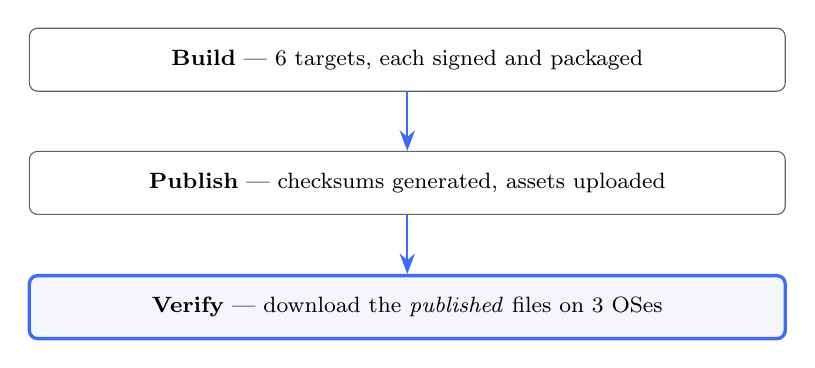
\begin{tikzpicture}[node distance=0.75cm and 1.2cm,
  box/.style={draw=krategrey, rounded corners=3pt, fill=white,
    minimum width=9.6cm, minimum height=0.8cm, align=left, font=\footnotesize},
  kbox/.style={draw=krateblue, very thick, rounded corners=3pt, fill=kratebg,
    minimum width=9.6cm, minimum height=0.8cm, align=left, font=\footnotesize},
  arrow/.style={-{Stealth[length=2.6mm]}, thick, draw=krateblue}]
  \node[box] (b) {\textbf{Build} --- 6 targets, each signed and packaged};
  \node[box, below=of b] (p) {\textbf{Publish} --- checksums generated, assets uploaded};
  \node[kbox, below=of p] (v) {\textbf{Verify} --- download the \emph{published} files on 3 OSes};
  \draw[arrow] (b) -- (p);
  \draw[arrow] (p) -- (v);
\end{tikzpicture}
\end{center}

The verify stage checks, on the real downloaded files:

\begin{itemize}[leftmargin=*]
  \item the checksum a careful person would check actually matches;
  \item the archive unpacks into a folder, not files with backslashes in
    their names (this check exists because we shipped that bug --- see
    Chapter 6);
  \item the binary reports the version on the tin;
  \item \texttt{cargo-component} ships beside it, so the build path works;
  \item the Windows document icon is present (K-058 shipped without it);
  \item macOS signing, entitlements and Gatekeeper pass (K-063, K-068);
  \item an app \emph{builds with the published binary and runs headless};
  \item \textbf{the permission wall still refuses without grants.}
\end{itemize}

\begin{factbox}{The sentence to use when someone doubts the quality}
``Every release downloads its own published files on three operating
systems and re-proves eight things about them, including that the
permission wall still refuses. Most of those checks exist because we
shipped that exact bug once.''
\end{factbox}

% =====================================================================
\chapter{The Numbers}

Every number in this chapter was measured on 11 August 2026 on an
M-series Mac, with the machine otherwise idle. Conditions are stated
because they change the answer.

\section{Speed}

\begin{center}
\begin{tabular}{lrp{6.6cm}}
\toprule
\textbf{Measurement} & \textbf{Result} & \textbf{What it means} \\
\midrule
Krate app launch, end to end & 11.3 ms & From typing the command to the app finishing \\
The same program, native binary & 5.0 ms & Compiled directly for this Mac \\
Ratio & 2.25$\times$ & Krate is about twice as slow to \emph{start} \\
\midrule
Runtime: compile + start a component & 3.3 ms & The engine's own work \\
Runtime: steady-state work & 61 $\mu$s & Once loaded, per invocation \\
\bottomrule
\end{tabular}
\end{center}

\begin{warnbox}{Do not claim Krate is faster than native}
It is not. It is roughly twice as slow to start a trivial program, and
that difference is a few milliseconds. What \emph{is} true and defensible:
there is no per-operation penalty. The overhead is a fixed startup cost of
a few milliseconds, not a tax that grows with the work. At 61 microseconds
of steady-state work, portability is costing nothing once running.
\end{warnbox}

\subsection{The honest sentence to use}

\begin{plainbox}{Say this}
``A Krate app starts in about 11 milliseconds --- roughly 6 milliseconds
behind the same program compiled natively, which nobody can perceive --- and
it is about 19 times smaller. After it starts there is no per-operation
cost at all.''
\end{plainbox}

\subsection{Where Krate genuinely wins on speed}

Against Electron, which is the real competition for cross-platform apps:
Electron apps typically take hundreds of milliseconds to start and occupy
80--200 MB. Krate starts in milliseconds at 15--30 KB. That comparison is
where the word ``faster'' is honest.

\section{Size}

\begin{center}
\begin{tabular}{lrr}
\toprule
\textbf{Thing} & \textbf{Size} & \textbf{Ratio vs Krate} \\
\midrule
Krate app (typical published) & 15--30 KB & 1$\times$ \\
Same program as a native binary & 336 KB & 19$\times$ larger \\
Typical Electron app & 80--200 MB & $\approx$5{,}000$\times$ larger \\
\midrule
The Krate runtime itself (installed once) & 21 MB & --- \\
\bottomrule
\end{tabular}
\end{center}

\begin{warnbox}{The honest caveat about the 21 MB}
The apps are tiny, but the runtime you install once is 21 MB. That is a
fair thing for a sceptic to point at. The answer: it is installed once and
shared by every app, so the tenth app you receive costs 20 KB, not another
21 MB. We have not yet audited what makes up those 21 MB --- turning off
the speech feature only saved 1 MB, so the common assumption that speech
is the bulk is wrong.
\end{warnbox}

\section{Reliability}

\begin{center}
\begin{tabular}{lr}
\toprule
\textbf{Measure} & \textbf{Value on 11 Aug 2026} \\
\midrule
Automated tests, all passing & 1{,}141 \\
Example apps in the repository & 39 \\
Example apps passing every check & 32 of 32 \\
Bugs recorded on the public board & 96 \\
Bugs fixed & 82 \\
Releases shipped & 36 \\
Platforms built and verified per release & 6 \\
\bottomrule
\end{tabular}
\end{center}

The six platforms are: macOS on Apple silicon, macOS on Intel, Windows on
Intel, Windows on ARM, Linux on Intel, and Linux on ARM. After each
release is published, a separate job downloads the published files on
three operating systems and verifies checksums, signatures, and that an
app actually builds and runs.

\section{The benchmark, stated honestly}

There is a benchmark of how often the AI produces a usable app. Its last
recorded run was 5 August 2026, and it scored \textbf{0 out of 5} on
authored apps under a strict ``did it do what was asked'' test.

\begin{warnbox}{This number is old and must be re-run}
Dozens of fixes have landed since that run, and apps written after it
(a tip calculator, a JSON formatter, a Markdown table tool, a Pomodoro
timer) do pass. But \textbf{we have not re-measured}, so there is no
current number. If someone asks ``what is your success rate'', the correct
answer is: ``the last honest measurement was before a lot of fixes and it
was bad; re-running it is on the list, and I will not quote a number I
have not measured.''
\end{warnbox}

That is uncomfortable, and it is deliberately in this document, because
quoting a number you cannot defend is worse than admitting you have not
measured it yet.

% =====================================================================
\chapter{How It Was Built}

\section{It was planned as an eight-phase, two-year project}

Krate was not built by improvising. Before the code, there were eight
written phase plans, each with a one-sentence objective, a duration, and
explicit success criteria. They are still in the repository. Here they are,
with the duration each was originally given:

\begin{center}
\begin{longtable}{clp{7.1cm}}
\toprule
& \textbf{Originally planned} & \textbf{The objective, in its own words} \\
\midrule
\endhead
0 & Weeks 1--4 & Get the project bones set up so real work can start \\
1 & Months 2--3 & Prove one \texttt{.wasm} runs identically on three desktop hosts \\
2 & 4--8 weeks & Ship the first useful cross-platform CLI app \\
3 & 6--10 weeks & First GUI app running natively on Windows, macOS and Linux \\
4 & Months 11--14 & The same \texttt{.krate} runs on iOS and Android without source changes \\
5 & Months 15--18 & A developer gets a working GUI app in under 60 seconds \\
6 & Months 19--22 & Users discover, install, update, and sign in across devices \\
7 & Months 23--24 & Launch quality, and ship v1.0 in public \\
\bottomrule
\end{longtable}
\end{center}

\begin{factbox}{The single most impressive fact in this document}
Phase 4 --- ``the same \texttt{.krate} runs on iOS and Android without
source changes'' --- was scheduled for \textbf{months 11 to 14}.

It ran on a real Android phone on 9 August 2026 and on a real iPhone on
10 August 2026, in month five.

The plan was not abandoned; it was beaten. Phases 0 through 3 are done, and
Phase 4's core proof landed roughly nine months ahead of its own schedule.
\end{factbox}

\section{The timeline of what actually happened}

\begin{center}
\begin{longtable}{lp{9.6cm}}
\toprule
\textbf{When} & \textbf{What happened} \\
\midrule
\endhead
April 2026 & Work begins, under the name Layer36. At this point there is no evidence that any of it is possible. \\
24 June 2026 & The status record begins. Three real command-line apps (\texttt{krate-clock}, \texttt{krate-cat}, \texttt{krate-curl}) run through the runtime. \\
2 July 2026 & Phase 2 formally closes out. The plan is amended rather than followed blindly. \\
\textbf{4 July 2026} & \textbf{The milestone.} All three desktop operating systems open a real native window from the same portable file, proven in one green CI run. \\
July 2026 & Renamed from Layer36 to Krate --- the previous name collided with other AI startups. The two-paths idea (receive vs.\ make) is set. \\
3 August 2026 & The current shipping repository's first commit. \\
5 August 2026 & Krate Cloud goes live; the first app is published from a terminal. \\
9 August 2026 & The Android player runs a real published app from a tapped link. \\
10 August 2026 & The iOS player runs on a real iPhone, under Pulley. GPU rendering added on Metal. \\
11 August 2026 & Seven numbered bugs (K-091 to K-097) fixed in one day; v0.1.10 and v0.1.11 ship. \\
\bottomrule
\end{longtable}
\end{center}

\begin{plainbox}{Why 4 July 2026 is the date that mattered}
Everything before it was a bet. One file, compiled once, opening a real
native window on macOS, Windows and Linux --- with a robot clicking the
button on Linux and the app noticing --- is the moment the central premise
stopped being a hypothesis. Every later achievement (the phones, the cloud,
the AI loop) is built on that one proof.
\end{plainbox}

\begin{plainbox}{What ``289 commits'' actually means}
The repository you can see today was started on 3 August 2026, so its
289 commits span eight days. That is the \emph{current} repository, not the
project. The work began in April under the name Layer36; the status record
runs from 24 June; the phase plans are older still; and the
three-operating-system proof was 4 July --- all before the first commit
here.

So when somebody points at the commit rate and implies the work is thin,
the accurate answer is: this is the shipping repository of a project that
started in April, and it moves fast because four phases of design and
proof were finished before any of this code was written.
\end{plainbox}

\section{What was genuinely uncertain}

It is worth being able to say what was \emph{not} known in April, because
the answer is: almost all of it.

\begin{itemize}[leftmargin=*]
  \item \textbf{Whether one binary could really draw a native window on
    three operating systems.} That was Phase 3's entire purpose, and it was
    a real question --- each system has a completely different windowing
    model.
  \item \textbf{Whether apps could be written without Rust's standard
    library.} Krate refuses operating-system calls, but ordinary Rust code
    pulls them in invisibly. This was unresolved until the \texttt{no\_std}
    guest work, and until it was solved, three out of eight AI-written apps
    failed for this reason alone.
  \item \textbf{Whether an AI could hit an API it had never seen.} There was
    no reason to assume yes. The answer turned out to depend less on the
    model than on having a checker that could say exactly what was wrong.
  \item \textbf{Whether the phones would work at all.} Phase 4 was over a
    year away in the plan and could have failed outright --- iOS forbids
    just-in-time compilation, which is how WebAssembly is normally made
    fast.
\end{itemize}

That last one deserves its own note, because it is the best engineering
answer in the project.

\begin{plainbox}{The iPhone problem, and the answer}
Apple does not permit an app to generate machine code while running. That
is exactly how a fast WebAssembly runtime normally works, so on paper
Krate could not run on an iPhone at all.

The answer was Pulley --- a portable interpreter --- instead of
just-in-time compilation. It was then verified to produce
\textbf{pixel-identical} output to the compiled path. The constraint was
real, the workaround was real, and it was checked rather than assumed.
\end{plainbox}

\section{The method: a public bug board}

Every defect found gets a number, an owner, a severity, and --- crucially
--- \emph{evidence}: the exact command and its output, not a description.
96 entries, 82 fixed.

The board also classifies who can fix each bug, which turns out to be the
most useful part:

\begin{center}
\begin{tabular}{lrp{7.6cm}}
\toprule
\textbf{Class} & \textbf{Count} & \textbf{Meaning} \\
\midrule
\texttt{our-code} & 67 & An ordinary defect in Krate \\
\texttt{example-bug} & 10 & Our example apps teach the bug, so every generated app inherits it \\
\texttt{runtime-hole} & 7 & The runtime cannot do it; no prompt helps \\
\texttt{environment} & 7 & This machine, not the product \\
\texttt{teaching-hole} & 4 & The runtime can do it and we never told the AI \\
\bottomrule
\end{tabular}
\end{center}

\begin{plainbox}{Why \texttt{example-bug} is the highest-leverage class}
An AI writing a Krate app reads our example apps to learn how. So a bug in
an example is not one bug --- it is a bug in every app anyone generates
afterwards. Ten entries are of this kind, and fixing one of them fixes
apps that have not been written yet.
\end{plainbox}

\section{Five real problems, and what they taught}

These are worth knowing in detail, because they are the honest story of
how the product got good, and they answer ``how do I know this is solid?''

\subsection{The 90-gigabyte memory leak}

A canvas game grew to 46 GB of memory when running in a window. The macOS
drawing code was creating a fresh image object every single frame and
never releasing them. Fixed by reusing one image view and draining the
memory pool each frame. Memory is now flat at about 80 MB.

\emph{Lesson: a bug that only appears in one mode (windowed, not headless)
will not be found by tests that never open a window.}

\subsection{Every Windows release shipped a broken zip file}

The ZIP file format specification requires forward slashes in paths.
Windows' own \texttt{Compress-\allowbreak Archive} writes backslashes.
Every Windows release we had ever shipped was technically malformed. It
was found only when we built a job that downloads the published files and
checks them.

\emph{Lesson: verifying what you published is different from verifying what
you built.}

\subsection{The app that was impossible to build}

An outside reviewer asked for a folder-tidying app and found it could not
exist: no app could name a folder, and no dialog existed to pick one, so
the AI reached for unrestricted filesystem access instead. He was right.
The answer was to invent ``the pick is the grant'' (Chapter 3), add it to
the runtime, and ship the app he described.

\emph{Lesson: when a reviewer says something is impossible, check whether
they are right before defending the design.}

\subsection{The product was slow, and it was not the runtime}

For months, a Krate app took 74 milliseconds to launch while the runtime
itself needed only 3.3. The other 91\% was Krate blocking every launch on
a telemetry message to our server. Fixed by writing the event to a file
and letting a separate process send it. Launches dropped from 74 ms to
6 ms.

\emph{Lesson: measure the whole path a person experiences, not the
component you are proud of.}

\subsection{Apps that closed their own windows}

Fifteen example apps ended their event loop after a fixed number of
rounds --- about thirty seconds of use --- so the window vanished while
somebody was using it. Including the app the AI is told to copy first.

\emph{Lesson: an example app is documentation. A bug in it is a bug in
everything written afterwards.}

% =====================================================================
\chapter{How the AI Part Works}

\section{Krate does not have its own AI}

This is the single most misunderstood point, and the answer is a strength,
not a weakness.

Krate does not train, host, or pay for any AI model. It drives whichever
AI coding tool you \emph{already have installed} --- Claude Code, Codex,
Gemini, Copilot, or Grok. If you pay one of them, you pay nothing extra to
Krate for authoring.

\begin{center}
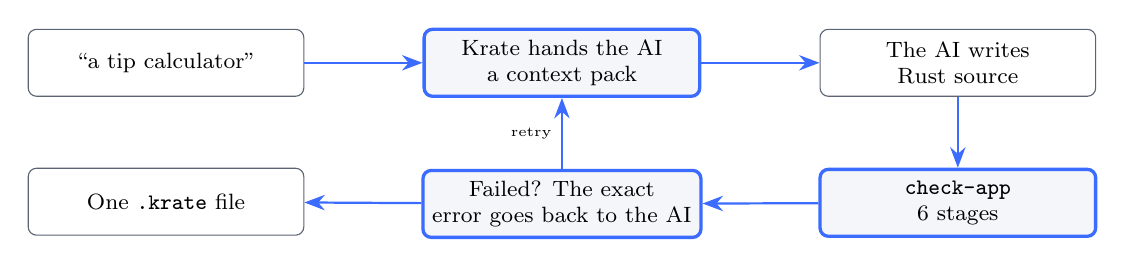
\begin{tikzpicture}[node distance=0.9cm and 1.5cm,
  box/.style={draw=krategrey, rounded corners=3pt, fill=white,
    minimum width=3.5cm, minimum height=0.85cm, align=center, font=\footnotesize},
  kbox/.style={draw=krateblue, very thick, rounded corners=3pt, fill=kratebg,
    minimum width=3.5cm, minimum height=0.85cm, align=center, font=\footnotesize},
  arrow/.style={-{Stealth[length=2.6mm]}, thick, draw=krateblue}]
  \node[box] (req) {``a tip calculator''};
  \node[kbox, right=of req] (pack) {Krate hands the AI\\a context pack};
  \node[box, right=of pack] (ai) {The AI writes\\Rust source};
  \node[kbox, below=of ai] (check) {\texttt{check-app}\\6 stages};
  \node[kbox, below=of pack] (loop) {Failed? The exact\\error goes back to the AI};
  \node[box, below=of req] (out) {One \texttt{.krate} file};
  \draw[arrow] (req) -- (pack);
  \draw[arrow] (pack) -- (ai);
  \draw[arrow] (ai) -- (check);
  \draw[arrow] (check) -- (loop);
  \draw[arrow] (loop) -- node[left,font=\tiny]{retry} (pack);
  \draw[arrow] (loop) -- (out);
\end{tikzpicture}
\end{center}

\section{The context pack: how the AI knows what to write}

An AI cannot guess an API it has never seen. So Krate generates a document
for it, freshly, from the actual source code: every callable function,
every capability name, the interface definitions, the discipline rules,
and an index of example apps by shape.

Because it is generated from the same source the runtime compiles, it
cannot drift out of date --- a class of failure that would otherwise
silently teach models an API that no longer exists. A test enforces this.

\section{The loop that makes it work}

The AI writes code. \texttt{check-app} judges it and, on failure, returns
the specific stage and a suggested fix. That goes back to the AI, which
tries again. The person sees none of this --- they see a progress line and
then a file.

\begin{plainbox}{Why this matters more than the model}
Any model writes broken code sometimes. What makes output trustworthy is
not a better model --- it is having a machine that can tell, definitively,
whether the code is acceptable, and can say exactly why not. That checker
is the actual product moat.
\end{plainbox}

\section{Honest limitations of the AI path}

\begin{itemize}[leftmargin=*]
  \item A build takes \textbf{5 to 12 minutes}, most of it compiling Rust.
  \item It sometimes needs a second attempt.
  \item The success rate has not been re-measured since 5 August (see
    Chapter 5).
  \item Authoring depends on other companies' tools, which can change.
    Supporting five providers is the mitigation.
\end{itemize}

% =====================================================================
\chapter{How Krate Compares}

\section{The comparison table}

\begin{center}
\begin{tabular}{lccccc}
\toprule
& \textbf{Krate} & \textbf{Electron} & \textbf{Flutter} & \textbf{Native} & \textbf{Web app} \\
\midrule
Size of one app & 15--30 KB & 80--200 MB & 10--40 MB & 1--20 MB & --- \\
One file, all systems & yes & rebuild & rebuild & no & n/a \\
Works offline as a file & yes & yes & yes & yes & no \\
Permission wall enforced & \textbf{yes} & no & no & OS-level & browser \\
Built for AI authorship & \textbf{yes} & no & no & no & no \\
Store approval to share & \textbf{none} & none & stores & stores & none \\
\bottomrule
\end{tabular}
\end{center}

\section{The gap nobody else fills}

Every existing option makes you choose:

\begin{itemize}[leftmargin=*]
  \item \textbf{Small and safe}, but not really yours --- a web app.
  \item \textbf{Real and installable}, but huge and unrestricted ---
    Electron or native.
\end{itemize}

Krate is a real file you own, tiny, and sandboxed by default. That
combination is the position.

\section{What about other WebAssembly runtimes?}

Wasmtime, Wasmer and WasmEdge are excellent engines --- Krate uses
wasmtime internally. But they are engines for servers and embedding, not
products for people. None of them gives you a double-clickable app file, a
permission wall in plain words, a window on three operating systems, an AI
authoring loop, or a publish-and-share link.

\analogy{Wasmtime is an engine. Krate is the car.}

% =====================================================================
\chapter{Where Krate Is Honestly Not Ready}

Volunteering this is the cheapest credibility available, and every item
here is something a sceptic would otherwise find.

\begin{enumerate}[leftmargin=*]
  \item \textbf{Smartphone players are days old.} Android and iOS both run
    real apps, but responsiveness on iPhone is still being tuned. They are
    not in any app store.
  \item \textbf{Not hardened against hostile code.} The wall stops honest
    apps from overreaching. It is not an adversarial security boundary and
    is never claimed as one.
  \item \textbf{Windows shows a SmartScreen warning.} macOS is fully
    signed and notarised; Windows needs a certificate we have not bought.
  \item \textbf{AI authoring takes 5--12 minutes} and sometimes needs a
    retry.
  \item \textbf{No heavy 3D or video.}
  \item \textbf{The authoring success rate has not been re-measured}
    since 5 August 2026.
  \item \textbf{The 21 MB runtime has not been audited} for what makes it
    that size.
  \item \textbf{One engineer.} The bug board, the goals file and the plan
    documents exist partly to make the work legible to someone else.
\end{enumerate}

% =====================================================================
\chapter{What Happens Next}

\section{The gates that define ``version 1''}

\begin{center}
\begin{tabular}{clp{6.6cm}}
\toprule
& \textbf{Gate} & \textbf{Status on 11 Aug 2026} \\
\midrule
G1 & A public, honest benchmark number & Harness exists; needs re-running \\
G2 & No blocker on the bug board & 82 of 96 fixed \\
G3 & Usability enforced, not hoped for & Done --- stage 6 of check-app \\
G4 & The outsider path works cold & Run once, defects found and fixed \\
G5 & Ten real people have made and sent an app & Not yet \\
\bottomrule
\end{tabular}
\end{center}

G5 is the only one that cannot be engineered around.

\section{The engineering queue}

\begin{enumerate}[leftmargin=*]
  \item Re-run the authoring benchmark and publish the number.
  \item Make generated apps look good by default --- the visual quality of
    an arbitrary new app is the current weak point.
  \item Finish smartphone responsiveness; port GPU rendering to Android.
  \item Windows code-signing certificate.
  \item Audit the 21 MB runtime.
\end{enumerate}

% =====================================================================
\chapter{Questions and Answers}

This chapter is written so you can answer anything, in the questioner's own
language, without preparation.

\section{From a normal person}

\textbf{``What is Krate, in one sentence?''}\\
An AI writes you a small app, and Krate turns it into one file that opens
on any computer and tells you what it wants before it runs.

\textbf{``Why should I care?''}\\
Because you can finally make a small tool for yourself --- a tracker, a
calculator, something for your mum's invoices --- and actually send it to
someone without them needing to install anything.

\textbf{``Is it safe to open a file a stranger made?''}\\
Safer than any normal program, because before it runs you see what it
wants and can refuse. An app that gets no permissions can genuinely do
nothing but draw in its own window.

\textbf{``Do I need to know how to code?''}\\
No. You type what you want in ordinary words.

\textbf{``Does it cost anything?''}\\
The runtime is free and open source, and publishing is free. You need one
AI coding tool, which most people who want this already pay for.

\section{From a developer}

\textbf{``Why WebAssembly rather than a scripting language?''}\\
Because Wasm is compiled (fast), portable (one file everywhere), and
sandboxed at the boundary rather than by convention. A Python script
cannot make the permission promise; a Wasm component can.

\textbf{``What is actually in the .krate file?''}\\
A zip containing the compiled WebAssembly component, the manifest, and
optionally assets and source.

\textbf{``How is the sandbox enforced?''}\\
The component can only call functions the runtime hands it. Every call
passes a guard that checks it against the session's granted capabilities.
Filesystem paths resolve inside the app's own directory with symlink and
containment checks; absolute paths and \texttt{\textasciitilde} are
refused at parse time.

\textbf{``What is the performance cost?''}\\
About 6 milliseconds more than native to start, and 61 microseconds of
steady-state work per invocation --- no per-operation tax. Numbers in
Chapter 5.

\textbf{``Why Rust for the apps?''}\\
Because it compiles to small, fast Wasm with no runtime of its own. The
person never writes it --- the AI does.

\textbf{``What is `no\_std' and why does it matter?''}\\
Rust's standard library assumes an operating system, and pulling it in
drags along calls Krate refuses. Apps are written without it, so they
import only Krate's own interfaces. \texttt{check-app} verifies this.

\textbf{``What happens when my app needs something Krate does not have?''}\\
Today, you cannot do it. That is a real limit, tracked on the board as
\texttt{runtime-hole}, and those are the entries we prioritise.

\section{From an investor}

\textbf{``What is the market?''}\\
Every person who will make software with AI and needs somewhere for it to
go. App stores were built for companies shipping to millions, not for a
tool with an audience of one.

\textbf{``Why now?''}\\
Because the making of software got solved in the last 18 months and the
delivering of it did not change at all.

\textbf{``What is defensible here?''}\\
Not the WebAssembly engine --- that is open source. What is hard to copy
is the verification loop (a machine that can tell whether AI-written code
is acceptable and why not), the capability model with plain-language
consent, and the six-platform delivery pipeline that verifies what it
published.

\textbf{``How much are you raising and what for?''}\\
Approximately \$750{,}000 on a SAFE. It funds roughly 18 months: the
founder full-time, the immigration path to the US, code-signing
certificates, cloud costs, and one senior engineer once the adoption loop
is proven.

\textbf{``How will the money be spent?''}
\begin{center}
\begin{tabular}{lr}
\toprule
\textbf{Use} & \textbf{Share} \\
\midrule
Founder salary, 18 months full-time & largest single line \\
One senior engineer, after adoption is proven & second largest \\
Immigration and relocation to the US & fixed cost \\
Code signing (Apple, Microsoft) and cloud & small, unavoidable \\
\bottomrule
\end{tabular}
\end{center}

\textbf{``What is the business model?''}\\
The runtime is free and open source; that is the adoption engine. Revenue
comes later from the cloud: private galleries, team distribution, and
usage beyond a free tier. Nothing is priced yet, deliberately --- adoption
first.

\textbf{``What are the traction numbers?''}\\
External testers, not users, as of 11 August 2026. The engineering is
ahead of the distribution, which is the honest position. Twelve apps are
published on the live gallery.

\section{The hard questions}

\textbf{``289 commits in eight days. Is this AI-generated slop?''}\\
The defence is not volume, it is verification: 1{,}141 automated tests, a
release pipeline that downloads its own published files on three operating
systems and re-verifies them, and a public bug board with 96 numbered
entries where the failures are documented with evidence. Judge the work by
what it survives, not by how fast it appeared.

\textbf{``What stops Apple, Microsoft or Google from doing this?''}\\
Nothing --- and if one of them does it, the thesis was right. What we have
is a working implementation, a public track record of fixing what real
people report, and no incentive to protect an existing app store.

\textbf{``Why hasn't anyone done this already?''}\\
The WebAssembly component model only became usable recently, and the
demand only exists because AI can now write apps for non-programmers. Both
halves are about two years old.

\textbf{``Your own benchmark said 0 out of 5.''}\\
It did, on 5 August 2026, under a deliberately strict test. That number is
in this document rather than hidden, and it drove the fixes that came
after. It has not been re-run, so we do not quote a better one.

\textbf{``You are one person. What happens if you are hit by a bus?''}\\
That is a real risk and the reason for the documentation discipline: the
bug board, the goals file, the plan documents, and this guide exist so the
work is legible to somebody else. The first engineering hire reduces it
further.

\textbf{``Is the permission wall real security?''}\\
It is real enforcement against honest apps that overreach --- the check
happens at the boundary, on every call. It is not hardened against
deliberately hostile code, and we say so everywhere rather than let
someone discover it.

\textbf{``Why would anyone trust an app a stranger's AI wrote?''}\\
They would not, and that is the point of the wall. You do not have to
trust the app. You only have to read four lines of plain English and
decide whether to allow them.

\section{Questions in the style of Y Combinator}

\textbf{``What do you do?''}\\
We make AI-written apps shareable. One small file, opens on any computer,
tells you what it wants first.

\textbf{``Who wants this urgently?''}\\
The person who just had an AI build them something useful and cannot give
it to anyone.

\textbf{``What have you learned from users?''}\\
That the failures are never where you expect. A tester hit a compiler
error and stopped --- which produced the two-paths design. A friend on
Windows found a generated game drawn off the screen --- which exposed that
21 of our own examples had the same defect and our own quality gate could
not see it. Both are in this document because both changed the product.

\textbf{``What is the one metric that matters?''}\\
Ten people who are not us making an app and sending it to someone. That is
gate G5, and it is not met yet.

% =====================================================================
\chapter{Glossary}

\begin{longtable}{lp{10.4cm}}
\toprule
\textbf{Term} & \textbf{Plain meaning} \\
\midrule
\endhead
WebAssembly (Wasm) & A portable form of compiled code that runs anywhere and can do nothing unless permitted \\
Runtime & The program that runs other programs; Krate is one \\
Component & One compiled Wasm app plus a description of what it needs \\
Capability & One specific power an app may ask for, e.g.\ ``open a window'' \\
Manifest & The file where an app declares what it wants, and why \\
Sandbox & A boundary an app cannot reach outside of \\
\texttt{.krate} & Krate's app file: a zip with the component, manifest and assets \\
Native & Compiled for one specific operating system and chip \\
Electron & A way of shipping web apps as desktop apps, by including a browser \\
Headless & Running without a visible window, for automated checks \\
\texttt{no\_std} & Writing Rust without its standard library, so no hidden OS calls appear \\
Component model & The WebAssembly standard for typed interfaces between a host and a guest \\
WIT & The language those interfaces are written in \\
Guest & The app running inside the runtime \\
Host & The runtime providing capabilities to the guest \\
\bottomrule
\end{longtable}

% =====================================================================
\chapter{Where Everything Lives}

\begin{center}
\begin{tabular}{lp{9cm}}
\toprule
\textbf{What} & \textbf{Where} \\
\midrule
The product & \url{https://krate.tech} \\
The source & \url{https://github.com/incyashraj/krate} \\
The cloud gallery & \url{https://krate.tech/cloud} \\
The bug board & \texttt{BUGS.md} in the repository \\
Direction and gates & \texttt{GOALS.md} \\
Verified claims for outreach & \texttt{Invest/OUTREACH\_TRUTH.md} \\
The development queue & \texttt{Plan/krate-dev-queue-2026-08.md} \\
This document & \texttt{Doc/krate-complete-guide.tex} \\
\bottomrule
\end{tabular}
\end{center}

\vspace{1cm}
\begin{factbox}{Keeping this document true}
Every figure here carries the date it was measured. When the numbers
change, change them here and change the date. A guide that quietly goes
stale is worse than no guide, because it makes you confident about
something that is no longer true.
\end{factbox}

\end{document}
